\documentclass[10pt,a4paper]{article}

\usepackage[spanish,activeacute,es-tabla]{babel}
\usepackage[utf8]{inputenc}
\usepackage{ifthen}
\usepackage{listings}
\usepackage{dsfont}
\usepackage{subcaption}
\usepackage{amsmath}
\usepackage[strict]{changepage}
\usepackage[top=1cm,bottom=2cm,left=1cm,right=1cm]{geometry}%
\usepackage{color}%
\newcommand{\tocarEspacios}{%
	\addtolength{\leftskip}{3em}%
	\setlength{\parindent}{0em}%
}

% Especificacion de procs

\newcommand{\In}{\textsf{in }}
\newcommand{\Out}{\textsf{out }}
\newcommand{\Inout}{\textsf{inout }}

\newcommand{\encabezadoDeProc}[4]{%
	% Ponemos la palabrita problema en tt
	%  \noindent%
	{\normalfont\bfseries\ttfamily proc}%
	% Ponemos el nombre del problema
	\ %
	{\normalfont\ttfamily #2}%
	\
	% Ponemos los parametros
	(#3)%
	\ifthenelse{\equal{#4}{}}{}{%
		% Por ultimo, va el tipo del resultado
		\ : #4}
}

\newenvironment{proc}[4][res]{%
	
	% El parametro 1 (opcional) es el nombre del resultado
	% El parametro 2 es el nombre del problema
	% El parametro 3 son los parametros
	% El parametro 4 es el tipo del resultado
	% Preambulo del ambiente problema
	% Tenemos que definir los comandos requiere, asegura, modifica y aux
	\newcommand{\requiere}[2][]{%
		{\normalfont\bfseries\ttfamily requiere}%
		\ifthenelse{\equal{##1}{}}{}{\ {\normalfont\ttfamily ##1} :}\ %
		\{\ensuremath{##2}\}%
		{\normalfont\bfseries\,\par}%
	}
	\newcommand{\asegura}[2][]{%
		{\normalfont\bfseries\ttfamily asegura}%
		\ifthenelse{\equal{##1}{}}{}{\ {\normalfont\ttfamily ##1} :}\
		\{\ensuremath{##2}\}%
		{\normalfont\bfseries\,\par}%
	}
	\renewcommand{\aux}[4]{%
		{\normalfont\bfseries\ttfamily aux\ }%
		{\normalfont\ttfamily ##1}%
		\ifthenelse{\equal{##2}{}}{}{\ (##2)}\ : ##3\, = \ensuremath{##4}%
		{\normalfont\bfseries\,;\par}%
	}
	\renewcommand{\pred}[3]{%
		{\normalfont\bfseries\ttfamily pred }%
		{\normalfont\ttfamily ##1}%
		\ifthenelse{\equal{##2}{}}{}{\ (##2) }%
		\{%
		\begin{adjustwidth}{+5em}{}
			\ensuremath{##3}
		\end{adjustwidth}
		\}%
		{\normalfont\bfseries\,\par}%
	}
	
	\newcommand{\res}{#1}
	\vspace{1ex}
	\noindent
	\encabezadoDeProc{#1}{#2}{#3}{#4}
	% Abrimos la llave
	\par%
	\tocarEspacios
}
{
	% Cerramos la llave
	\vspace{1ex}
}

\newcommand{\aux}[4]{%
	{\normalfont\bfseries\ttfamily\noindent aux\ }%
	{\normalfont\ttfamily #1}%
	\ifthenelse{\equal{#2}{}}{}{\ (#2)}\ : #3\, = \ensuremath{#4}%
	{\normalfont\bfseries\,;\par}%
}

\newcommand{\pred}[3]{%
	{\normalfont\bfseries\ttfamily\noindent pred }%
	{\normalfont\ttfamily #1}%
	\ifthenelse{\equal{#2}{}}{}{\ (#2) }%
	\{%
	\begin{adjustwidth}{+2em}{}
		\ensuremath{#3}
	\end{adjustwidth}
	\}%
	{\normalfont\bfseries\,\par}%
}

% Tipos

\newcommand{\nat}{\ensuremath{\mathds{N}}}
\newcommand{\ent}{\ensuremath{\mathds{Z}}}
\newcommand{\float}{\ensuremath{\mathds{R}}}
\newcommand{\bool}{\ensuremath{\mathsf{Bool}}}
\newcommand{\cha}{\ensuremath{\mathsf{Char}}}
\newcommand{\str}{\ensuremath{\mathsf{String}}}

% Logica

\newcommand{\True}{\ensuremath{\mathrm{true}}}
\newcommand{\False}{\ensuremath{\mathrm{false}}}
\newcommand{\Then}{\ensuremath{\rightarrow}}
\newcommand{\Iff}{\ensuremath{\leftrightarrow}}
\newcommand{\implica}{\ensuremath{\longrightarrow}}
\newcommand{\IfThenElse}[3]{\ensuremath{\mathsf{if}\ #1\ \mathsf{then}\ #2\ \mathsf{else}\ #3\ \mathsf{fi}}}
\newcommand{\yLuego}{\land _L}
\newcommand{\oLuego}{\lor _L}
\newcommand{\implicaLuego}{\implica _L}

\newcommand{\cuantificador}[5]{%
	\ensuremath{(#2 #3: #4)\ (%
		\ifthenelse{\equal{#1}{unalinea}}{
			#5
		}{
			$ % exiting math mode
			\begin{adjustwidth}{+2em}{}
				$#5$%
			\end{adjustwidth}%
			$ % entering math mode
		}
		)}
}

\newcommand{\existe}[4][]{%
	\cuantificador{#1}{\exists}{#2}{#3}{#4}
}
\newcommand{\paraTodo}[4][]{%
	\cuantificador{#1}{\forall}{#2}{#3}{#4}
}

%listas

\newcommand{\TLista}[1]{\ensuremath{seq \langle #1\rangle}}
\newcommand{\lvacia}{\ensuremath{[\ ]}}
\newcommand{\lv}{\ensuremath{[\ ]}}
\newcommand{\longitud}[1]{\ensuremath{|#1|}}
\newcommand{\cons}[1]{\ensuremath{\mathsf{addFirst}}(#1)}
\newcommand{\indice}[1]{\ensuremath{\mathsf{indice}}(#1)}
\newcommand{\conc}[1]{\ensuremath{\mathsf{concat}}(#1)}
\newcommand{\cab}[1]{\ensuremath{\mathsf{head}}(#1)}
\newcommand{\cola}[1]{\ensuremath{\mathsf{tail}}(#1)}
\newcommand{\sub}[1]{\ensuremath{\mathsf{subseq}}(#1)}
\newcommand{\en}[1]{\ensuremath{\mathsf{en}}(#1)}
\newcommand{\cuenta}[2]{\mathsf{cuenta}\ensuremath{(#1, #2)}}
\newcommand{\suma}[1]{\mathsf{suma}(#1)}
\newcommand{\twodots}{\ensuremath{\mathrm{..}}}
\newcommand{\masmas}{\ensuremath{++}}
\newcommand{\matriz}[1]{\TLista{\TLista{#1}}}
\newcommand{\seqchar}{\TLista{\cha}}

\renewcommand{\lstlistingname}{Código}
\lstset{% general command to set parameter(s)
	language=Java,
	morekeywords={endif, endwhile, skip},
	basewidth={0.47em,0.40em},
	columns=fixed, fontadjust, resetmargins, xrightmargin=5pt, xleftmargin=15pt,
	flexiblecolumns=false, tabsize=4, breaklines, breakatwhitespace=false, extendedchars=true,
	numbers=left, numberstyle=\tiny, stepnumber=1, numbersep=9pt,
	frame=l, framesep=3pt,
	captionpos=b,
}

\usepackage{caratula} % Version modificada para usar las macros de algo1 de ~> https://github.com/bcardiff/dc-tex


\titulo{Descripci\'on del tp}
\subtitulo{Subtítulo del tp}

\fecha{\today}

\materia{Materia de la carrera}
\grupo{Grupo 42}

\integrante{Krivonosoff, Thiago}{310/24}{thiagokribas@gmail.com}
\integrante{Pelli, Agustin}{002/01}{email2@dominio.com}
\integrante{Miguel, Facundo}{003/01}{email3@dominio.com}
\integrante{Montenegro, Ulises}{477/24}{ulinicolasmonte@gmail.com}
% Pongan cuantos integrantes quieran

% Declaramos donde van a estar las figuras
% No es obligatorio, pero suele ser comodo
\graphicspath{{../static/}}

\begin{document}

\maketitle

\section{Ejemplo de sección}
\subsection{Subsección: ambientes comunes de \LaTeX}

Lo principal: las fórmulas. Se puede poner en una linea, como $x_i = x_{i-1} + x_{i-2}$, o ponerse más grande:

\begin{equation}
	\sum\limits_{i=0}^{n} i
	\label{eq:1}
\end{equation}

Y se pueden citar ecuaciones con \verb|\eqref{nombreDeEq}|: \eqref{eq:1}

Ejemplo de itemizado:

\begin{itemize}
	\item Item 1
	\item Item 2
	\item Item 3
\end{itemize}

Ejemplo de enumerado con menor distancia entre items:

\begin{enumerate} \setlength\itemsep{0cm}
	\item Item 1
	\item Item 2
	\item Item 3
\end{enumerate}

Podemos escribir mucho texto. Mucho texto. Mucho texto. Mucho texto. Mucho texto. Mucho texto. Mucho texto. Mucho texto. Mucho texto. Mucho texto. Mucho texto.

Otro párrafo. Otro párrafo. Otro párrafo. Otro párrafo. Otro párrafo. Otro párrafo. Otro párrafo. Otro párrafo. Otro párrafo. Otro párrafo. Otro párrafo. Otro párrafo. Otro párrafo.

\vspace{0.3cm}

Le agregamos una separación entre párrafos. Le agregamos una separación entre párrafos. Le agregamos una separación entre párrafos. Le agregamos una separación entre párrafos. Le agregamos una separación entre párrafos.

\vspace{0.3cm}

La tabla \ref{tab:ejemplo} es un ejemplo de cómo se hace una tabla.

\begin{table}[h!]
	\centering
	\begin{tabular}{||l c c r||} 
		\hline
		Col1 & Col2 & Col2 & Col3 \\ [0.5ex] 
		\hline\hline
		1 & 6 & 87837 & 787 \\ 
		2 & 7 & 78 & 5415 \\
		3 & 545 & 778 & 7507 \\
		4 & 545 & 18744 & 7560 \\
		5 & 88 & 788 & 6344 \\
		\hline
	\end{tabular}
	\caption{Ejemplo de tabla}
	\label{tab:ejemplo}
\end{table}


La figura \ref{fig:subfigs} es un ejemplo de cómo se agrega una imagen.

\begin{figure}[ht]
	\centering
	
\includegraphics[width=0.6\textwidth]{logo_dc.jpg}
	\caption{Ejemplo de figura}
	\label{fig:ejemplo}
\end{figure}

\begin{figure}[ht!]
	\begin{subfigure}{0.5\textwidth}
		
\includegraphics[width=0.9\linewidth]{LaTeX-project} 
		\caption{Logo de LaTeX}
		\label{fig:subfig1}
	\end{subfigure}
	\begin{subfigure}{0.5\textwidth}
		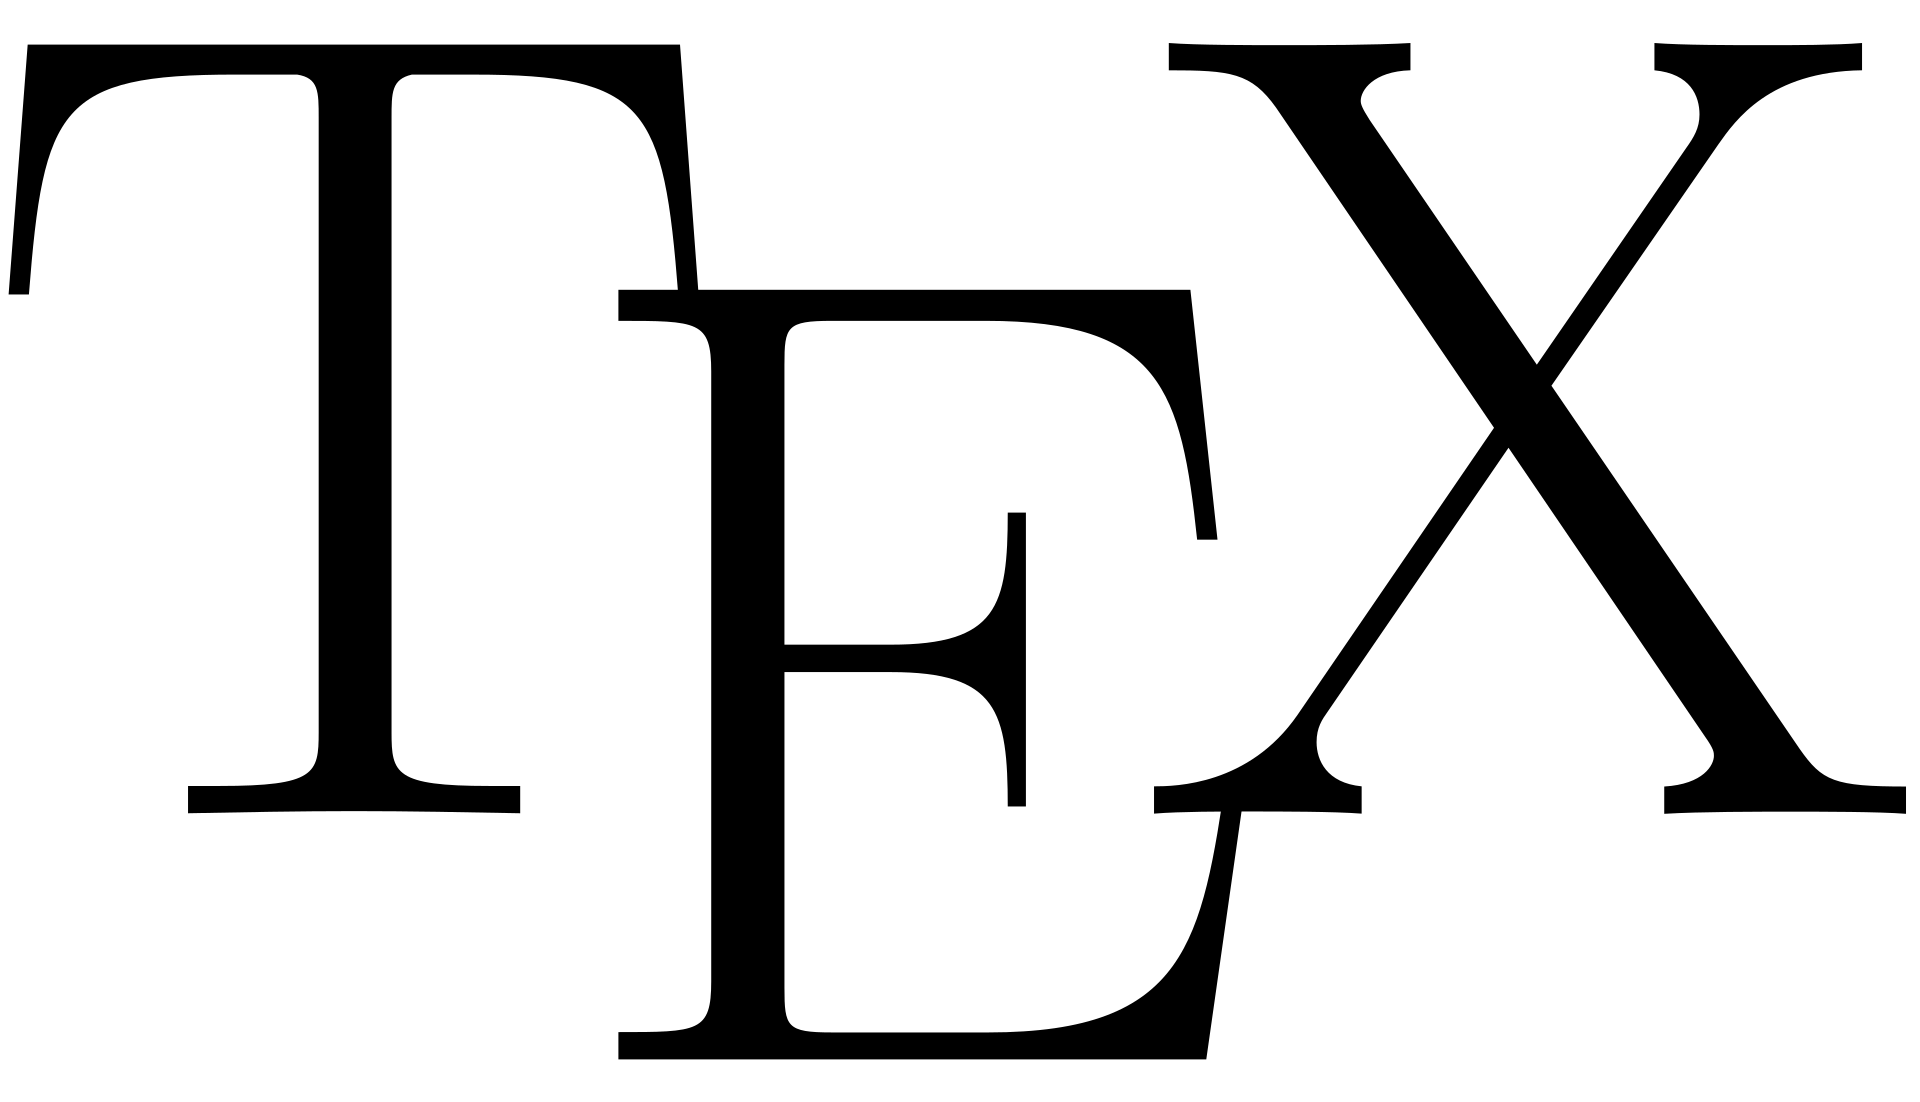
\includegraphics[width=0.7\linewidth]{TeX}
		\caption{Logo de TeX}
		\label{fig:subfig2}
	\end{subfigure}
	\caption{Ejemplo para poner dos figuras juntas. Y citarlas por separado a (\subref{fig:subfig1}) y (\subref{fig:subfig2}).}
	% OJO: el caption siempre va antes del label
	\label{fig:subfigs}
\end{figure}



% Para hacer que quede todo en una misma linea, se puede usar minipage
%\begin{minipage}[t]{\textwidth}
	\begin{lstlisting}[caption={Ejemplo de código (usando los estilos de la cátedra, ver las macros para más detalles)},label=code:for]
res := 0;
i := 0;
while (i < s.size()) do
	res := res + s[i];
	i := i + 1
endwhile
	\end{lstlisting}
%\end{minipage}

Si se pone un label al \verb|lstlisting|, se puede referenciar: Código \ref{code:for}.


\subsection{Macros de la cátedra para especificar}

\begin{proc}{nombre}{\In paramIn : \nat, \Inout paramInout : \TLista{\ent}}{tipoRes}
	%    \modifica{parametro1, parametro2,..}
	\requiere{expresionBooleana1}
	\asegura{expresionBooleana2}
	\aux{auxiliar1}{parametros}{tipoRes}{expresion}
	\pred{pred1}{parametros}{expresion} 
\end{proc}

\aux{auxiliarSuelto}{parametros}{tipoRes}{expresion}
% \paraTodo{variable}{tipo}{expresion}
% \existe{variable}{tipo}{expresion}
% Pueden tener [unalinea] para que no se divida en varias lineas
\pred{predSuelto}{parametros}{\paraTodo[unalinea]{variable}{tipo}{algo \implicaLuego expresion}}
\pred{predSuelto}{parametros}{\existe[unalinea]{variable}{tipo}{algo \yLuego expresion}}


A partir de aca empieza el TP.

%salto de lineas

\section{Problema 1}

\begin{proc}{grandesCiudades}{\In ciudades : \TLista{Ciudad}}{\TLista{Ciudad}}
	\requiere{noRepetidos(ciudades) \land noHabitantesNegativos(ciudades)}
	\asegura{ \longitud{res} \leq \longitud{ciudades} }
	\asegura{ \paraTodo[unalinea]{elem}{Ciudad}{(elem.habitantes > 50000 \land elem \in ciudades) \implica elem \in res}}
\end{proc}

\pred{noRepetidos}{\In ciudades: \TLista{Ciudad}}
	{\paraTodo[unalinea]{i}{\ent}{0 \leq i < |ciudades|}\implicaLuego \paraTodo[unalinea]{j}{\ent}{0 \leq j < |ciudades|}\implicaLuego (i \neq j \implica ciudades[i].nombre \neq ciudades[j].nombre)}

\pred{noHabitantesNegativos}{\In ciudades: \TLista{Ciudad}}
	{\paraTodo[unalinea]{i}{\ent}{0 \leq i < |ciudades|} \implicaLuego ciudades[i].habitantes >= 0}

\section{Problema 2}

\begin{proc}{sumaDeHabitantes}{\In menoresDeCiudades: \TLista{Ciudad}, \In mayoresDeCiudades: \TLista{Ciudad}}{\TLista{Ciudad}}
	\requiere{noRepetidos(menoresDeCiudades) \land noRepetidos(mayoresDeCiudades)}
	\requiere{noHabitantesNegativos(menoresDeCiudades) \land noHabitantesNegativos(mayoresDeCiudades)} 
	\requiere{mismosElementos(menoresDeCiudades, mayoresDeCiudades)}
	\requiere{|menoresDeCiudades| = |mayoresDeCiudades|}
	\asegura{|res| = |mayoresDeCiudades|}
	\asegura{\paraTodo[unalinea]{elem}{Ciudad}{(elem \in res) \implica  \\ 
	{\paraTodo[unalinea]{i}{\ent}{0 \leq i < |res|}\implicaLuego \existe[unalinea]{j}{\ent}{0 \leq j < |res|}}}
		\yLuego \\
		{mayoresDeCiudades[i].nombre = menoresDeCiudades[j].nombre} \implica \\
		res[i].nombre = mayoresDeCiudades[i].nombre \land \\
		res[i].habitantes = mayoresDeCiudades[i].habitantes + menoresDeCiudades[j].habitantes}
\end{proc}
\newpage

\pred{mismosElementos}{\In s1: \TLista{Ciudad}, \In s2: \TLista{Ciudad}}{
	{\paraTodo[unalinea]{i}{\ent}{0 \leq i < |s1|} \implicaLuego \existe[unalinea]{j}{\ent}{0 \leq j < |s1|} \yLuego s1[i].nombre = s2[j].nombre}
}

\section{Problema 3}

\begin{proc}{hayCamino}{\In distancia: \TLista{\TLista{\ent}}, \In desde: \ent, \In hasta: \ent}{\bool}
	\requiere{esCuadrada(distancia)}
	\requiere{0 \leq desde < |distancia|}
	\requiere{0 \leq hasta < |distancia|}
	\requiere{filaIgualColumna(distancia)}
	\requiere{matrizTodosPositivos(distancia)}
	\asegura{\existe[unalinea]{sec}{\TLista{\ent}}{|sec| > 1} \land \paraTodo[unalinea]{i}{\ent}{0 \leq i < |sec|} \implicaLuego \\ 	0 \leq sec[i] < |distancia| \land sec[0] = desde \land sec[|sec|-1] = hasta \land \\
	todosConexionAnterior(sec, distancia)}

\end{proc}

\pred{todosConexionAnterior}{\In sec: \TLista{\ent}, \In mat: \TLista{\TLista{\ent}}}{
	\paraTodo[unalinea]{j}{\ent}{1 \leq i < |sec| \implicaLuego mat[sec[i]][sec[i-1]] \neq 0
}}
\pred{esCuadrada}{\In mat: \TLista{\TLista{\ent}}}{
	\paraTodo[unalinea]{i}{\ent}{0 \leq i < |mat|} \implicaLuego |mat| = |mat[i]|
}\\
\pred{filaIgualColumna}{\In mat: \TLista{\TLista{\ent}}}{
	\paraTodo[unalinea]{i}{\ent}{0 \leq i < |mat|} \implicaLuego \paraTodo[unalinea]{j}{\ent}{0 \leq j < |mat|} \implicaLuego mat[i][j] = mat[j][i]
}\\
\pred{matrizTodosPositivos}{\In mat: \TLista{\TLista{\ent}}}{
	\paraTodo[unalinea]{i}{\ent}{0 \leq i < |mat|} \implicaLuego \paraTodo[unalinea]{j}{\ent}{0 \leq j < |mat|} \implicaLuego mat[i][j] >= 0
}\\
\section{Problema 4}

\begin{proc}{cantidadCaminosNSaltos}{\Inout conexion: \TLista{\TLista{\ent}}, \In n: \ent}{}
	\requiere{1 \leq n}
        \requiere{esCuadrada(conexion)}
	\requiere{filaIgualColumna(conexion)}
	\requiere{\paraTodo[unalinea]{i}{\ent}{0 \leq i < |conexion|} \implicaLuego \paraTodo[unalinea]{j}{\ent}{0 \leq j < |conexion|} \implicaLuego conexion[i][j] \in [0,1]}
	\requiere{conexion = C_0}
	\asegura{\existe[unalinea]{sec}{\TLista{\TLista{\TLista{\ent}}}}{|sec| = n} \land sec[0] = C_0 \land\\
	\paraTodo[unalinea]{i}{\ent}{1 \leq i < |sec|} \implicaLuego sec[i] = multiplicarMatrices(C_0, sec[i-1]) \implica conexion = sec[|sec| - 1] }
\end{proc}

\aux{inversa}{\In mat: \TLista{\TLista{\ent}}}{\TLista{\TLista{\ent}}}{\\
\paraTodo[unalinea]{i}{\ent}{0 \leq i < |mat|}\implicaLuego \paraTodo[unalinea]{j}{\ent}{0 \leq j < |mat|} \implicaLuegos res[j][i] = mat[i][j]
}

\aux{multiplicarMatrices}{\In mat1: {\TLista{\TLista{\ent}}}, \In mat2: {\TLista{\TLista{\ent}}}}{\TLista{\TLista{\ent}}}{\\
	\paraTodo[unalinea]{i}{\ent}{0 \leq i < |mat1|}\implicaLuego \paraTodo[unalinea]{j}{\ent}{0 \leq j < |mat1[i]|} \implicaLuego \\
	res[i][j] = productoEscalar(mat1[i], inversa(mat2)[j])
}

\aux{productoEscalar}{\in fila: \TLista{\ent}, \in col: \TLista{\ent}}{\ent}{\\
	\paraTodo[unalinea]{i}{\ent}{0 \leq i < |fila|} \implicaLuego \paraTodo[unalinea]{j}{\ent}{0 \leq j < |col|} \implicaLuego res = \sum_{i = 0}^{|fila| - 1} fila[i] * fila[j]
}

\section{Punto 2.1}
\subtitle{Demostramos que la implementación es correcta con correcta con respecto a la especificación dada mediante teorema de invariante y teorema de terminación.}

Por teorema del invariante primero debemos demostrar los siguientes puntos:

I = 0 \leq i \leq |\text{ciudades}| \land \sum_{j=0}^{i-1} \text{ciudades}[j].habitantes = res

\begin{itemize}
    \item \( P_c \implica I \)
    \item \( \{I \land B\} \ S \ \{I\} \)
    \item \( I \land \neg B \implica Q_c \)
\end{itemize}

\textbf{Primer paso} Probamos primero la implicación de la precondición del ciclo hacia el invariante:

P_c \implica I

\[
res = 0 \land i = 0 \implica 0 \leq i \leq |\text{ciudades}| \land \sum_{j=0}^{i-1} \text{ciudades}[j].habitantes = res
\]

\[
 0 \leq 0 \leq |\text{ciudades}| \land \sum_{j=0}^{0-1} \text{ciudades}[j].habitantes = 0
\]

\[
True \land True
\]

\[
True
\]

\textbf{Segundo paso} Ahora probamos que vale la siguiente tripla de Hoare:

\{I \land B\} \ S \ \{I\}

Hacemos uso del axioma.

\[
wp(S, I) \cong wp(S_1, wp(S_2, I))
\]

\[
wp(S_2, I) \cong def(S_2) \yLuego I_i^{i := i+1}
\]

\[
wp(S_2, I) \cong True \land 0 \leq i+1 \leq |\text{ciudades}| \yLuego \sum_{j=0}^{i} \text{ciudades}[j].habitantes = res
\]

Terminamos de definir el wp de S2:

\[
wp(S_2, I) \cong 0 \leq i+1 \leq |\text{ciudades}| \yLuego \sum_{j=0}^{i} \text{ciudades}[j].habitantes = res
\]

Ahora definimos el wp de S1:

\[
wp(S_1, wp(S_2, I)) \cong wp(res = res + \text{ciudades}[i].habitantes, 0 \leq i+1 \leq |\text{ciudades}| \yLuego \sum_{j=0}^{i} \text{ciudades}[j].habitantes = res)
\]

\[
wp(S_1, wp(S_2, I)) \cong def(res = res + \text{ciudades}[i].habitantes) \yLuego I_res^{res + \text{ciudades}[i].habitantes}
\]

\[
wp(S_1, wp(S_2, I)) \cong True \yLuego 0 \leq i+1 \leq |\text{ciudades}| \yLuego \sum_{j=0}^{i} \text{ciudades}[j].habitantes = res + \text{ciudades}[i].habitantes
\]

\[
wp(S_1, wp(S_2, I)) \cong 0 \leq i+1 \leq |\text{ciudades}| \yLuego \sum_{j=0}^{i} \text{ciudades}[j].habitantes = res + \text{ciudades}[i].habitantes
\]

Ahora queda definido el wp de S:

\[
wp(S, I) \cong 0 \leq i < |\text{ciudades}| \yLuego \sum_{j=0}^{i-1} \text{ciudades}[j].habitantes = res
\]

Ahora veo la implicacion del invariante y la guarda hacia wp(S,I):

\[
\{I \land B\} \implica wp(S, I) \cong (sigue abajo)
\]

\[
 0 \leq i < |\text{ciudades}| \land 0 \leq i \leq |\text{ciudades}| \yLuego \sum_{j=0}^{i-1} \text{ciudades}[j].habitantes = res \implica (sigue abajo)
\]

\[
0 \leq i < |\text{ciudades}| \yLuego \sum_{j=0}^{i-1} \text{ciudades}[j].habitantes = res
\]

Se cancelan los terminos y queda:

\[
0 \leq i \leq |\text{ciudades}| \implica True
\]

\[
True
\]

\textbf{Tercer paso} Ahora probamos que vale la siguiente implicación:
\( I \land \neg B \implica Q_c \)

\[
0 \leq i \leq |\text{ciudades}| \yLuego \sum_{j=0}^{i-1} \text{ciudades}[j].habitantes = res \land i \geq |\text{ciudades}| (sigue abajo)
\]

\[
\implica \sum_{j=0}^{|\text{ciudades}|-1} \text{ciudades}[j].habitantes = res \land i = |\text{ciudades}|
\]

Se cancelan las sumatorias y la igualdad

\[
0 \leq i \leq |\text{ciudades}| \implica True
\]

\[
True
\]

Ahora por teorema de terminación ahora debemos demostrar que la ejecucion del ciclo siempre termina, nuestra función variante:

\textbf{F_v = |\text{ciudades}| - i - 1}

\begin{itemize}
    \item \( \{ I \land B \land F_v = v_0\} S \{ F_v < v_0 \} \)
    \item \( I \land F_v \leq 0 \implica \neg B \)
\end{itemize}

\textbf{Primer paso} Probamos la primera implicación:

\{ I \land B \land F_v = v_0\} S \{ F_v < v_0 \}

\[
\{0 \leq i \leq |\text{ciudades}| \yLuego \sum_{j=0}^{i-1} \text{ciudades}[j].habitantes = res \land 0 \leq i \leq |\text{ciudades}| \land F_v = |\text{ciudades}| - i - 1\} \implica (sigue abajo)
\]

\[
wp(S, F_v < v_0) =
\]

\[
wp(S1, wp(S2, F_v < v_0)) =
\]

\[
wp(S1, wp(i:=i+1, F_v < v_0)) =
\]

\[
wp(S1, True \land F_v = |\text{ciudades}| - i - 2 < v_0) =
\]

\[
wp(res:= res + \text{ciudades}[i].habitantes, True \land F_v = |\text{ciudades}| - i - 2 < v_0) = 
\]

\[
True \land F_v = |\text{ciudades}| - i - 1 < v_0 =
\]

\[
F_v = |\text{ciudades}| - i - 1 < v_0
\]

Finalmente la implicación nos queda de la forma

\[
\{0 \leq i \leq |\text{ciudades}| \yLuego \sum_{j=0}^{i-1} \text{ciudades}[j].habitantes = res \land 0 \leq i \leq |\text{ciudades}| \land F_v = |\text{ciudades}| - i - 1\} \implica (sigue abajo)
\]

\[
|\text{ciudades}| - i - 1 < |\text{ciudades}| - i 
\]

Se cancelan los terminos y queda

\[
\{0 \leq i \leq |\text{ciudades}| \yLuego \sum_{j=0}^{i-1} \text{ciudades}[j].habitantes = res \yLuego F_v = |\text{ciudades}| - i - 1 \} \implica True
\]

\[
True
\]

\textbf{Segundo paso} Probamos la segunda implicación:

I \land F_v \leq 0 \implica \neg B

\[
0 \leq i \leq |\text{ciudades}| \yLuego res = \sum_{j=0}^{i-1} \text{ciudades}[j].habitantes \yLuego |\text{ciudades}| - i - 1 \leq 0 \implica i \geq |\text{ciudades}|
\]

\[
0 \leq i \leq |\text{ciudades}| \land |\text{ciudades}| \leq i + 1 \implica i \geq |\text{ciudades}|
\]

\[
i = |\text{ciudades}| \implica i \geq |\text{ciudades}|
\]

\[
True
\]

\section{Ejercicio 2.2}

Teniendo en cuenta la correctitud del programa demostrada en el 2.1, sabemos que el valor devuelto por el programa, siempre que se cumpla la precondición, tendrá la pinta de:

\[
\text{res} = \text{sumatoria}  
\]

En el procedimiento, se especifica que el parámetro de entrada es de tipo IN, por lo tanto en la precondición y la postcondición, el parámetro \textit{ciudades} mantendrá las mismas características, entre ellas que sus elementos son todos mayores o iguales a 0. Por lo tanto, al tomar un elemento de \textit{ciudades}, obligatoriamente será menor o igual a la sumatoria del total de elementos de \textit{ciudades}, es decir:

\[
\textit{ciudades}[i].habitantes \leq \text{sumatoria} \text{con algún i} 0 \leq i < |\textit{ciudades}|
\]

Ahora bien, según la postcondición sabemos que \text{res} = la sumatoria de todos sus elementos, entre los cuales sabemos que al menos alguno de ellos es mayor a 50.000, por lo tanto:

\[
50.000 < \textit{ciudades}[k].habitantes \quad \text{con algún k} \quad 0 \leq k < |\textit{ciudades}|
\]

Podemos afirmar entonces que:

\[
50.000 < \textit{ciudades}[k].habitantes \leq \text{sumatoria} \quad \text{con algún k} \quad 0 \leq k < |\textit{ciudades}|
\]

Y por transitividad concluimos que:

\[
50.000 < \text{sumatoria}
\]

\end{document}
